\section{Scalar Hyperbolic Problem}
\subsection{Convergence Analysis}
\begin{table}[H]
	\centering
	\begin{tabular}{|c|c|c|c|}
		\hline
		$N$  & Second Order          & Fourth Order          & Fourier                \\
		\hline
		8    & $1.73 \times 10^{0}$  & $6.37 \times 10^{-1}$ & $8.25 \times 10^{-4}$  \\
		16   & $1.06 \times 10^{0}$  & $2.02 \times 10^{-1}$ & $7.45 \times 10^{-6}$  \\
		32   & $4.41 \times 10^{-1}$ & $2.14 \times 10^{-2}$ & $5.25 \times 10^{-7}$  \\
		64   & $1.32 \times 10^{-1}$ & $1.41 \times 10^{-3}$ & $3.54 \times 10^{-8}$  \\
		128  & $3.26 \times 10^{-2}$ & $9.17 \times 10^{-5}$ & $2.30 \times 10^{-9}$  \\
		256  & $8.06 \times 10^{-3}$ & $5.83 \times 10^{-6}$ & $1.47 \times 10^{-10}$ \\
		512  & $2.01 \times 10^{-3}$ & $3.68 \times 10^{-7}$ & $1.16 \times 10^{-11}$ \\
		1024 & $5.03 \times 10^{-4}$ & $2.31 \times 10^{-8}$ & $5.51 \times 10^{-12}$ \\
		2048 & $1.26 \times 10^{-4}$ & $1.45 \times 10^{-9}$ & $1.05 \times 10^{-11}$ \\
		\hline
	\end{tabular}
	\caption{$L_{\infty}$-Error for the Scalar Hyperbolic Problem at $t = \pi$}
	\label{tab:hyperbolic_error}
\end{table}

\begin{table}[H]
	\centering
	\begin{tabular}{|c|c|c|c|}
		\hline
		$N$  & Second Order & Fourth Order & Fourier \\
		\hline
		16   & 0.71         & 1.66         & 6.79    \\
		32   & 1.26         & 3.24         & 3.83    \\
		64   & 1.75         & 3.92         & 3.89    \\
		128  & 2.01         & 3.94         & 3.95    \\
		256  & 2.01         & 3.97         & 3.96    \\
		512  & 2.00         & 3.99         & 3.66    \\
		1024 & 2.00         & 3.99         & 1.08    \\
		2048 & 2.00         & 3.99         & -0.92   \\
		\hline
	\end{tabular}
	\caption{Convergence Rates for the Scalar Hyperbolic Problem}
	\label{tab:hyperbolic_rates}
\end{table}

\subsection{Longterm Convergence}

\begin{figure}[H]
	\centering
	\begin{subfigure}{0.5\textwidth}
		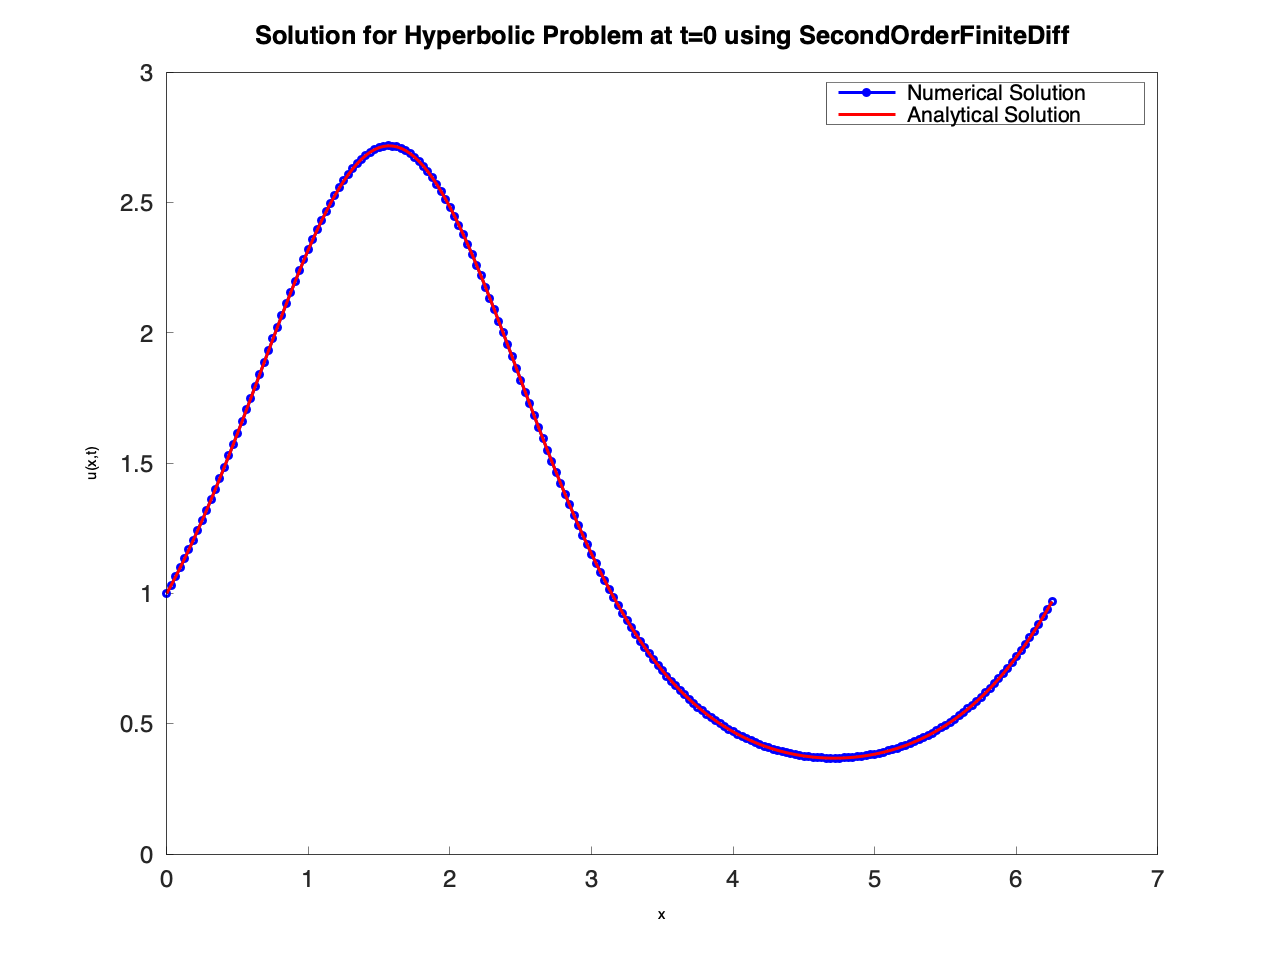
\includegraphics[width=\textwidth]{media/hyperbolic_SecondOrderFiniteDiff_0.png}
		\caption{Second Order at $t=0$ with $L_\infty=0.0$}
		\label{sfig:sublabel1}
	\end{subfigure}%
	~
	\begin{subfigure}{0.5\textwidth}
		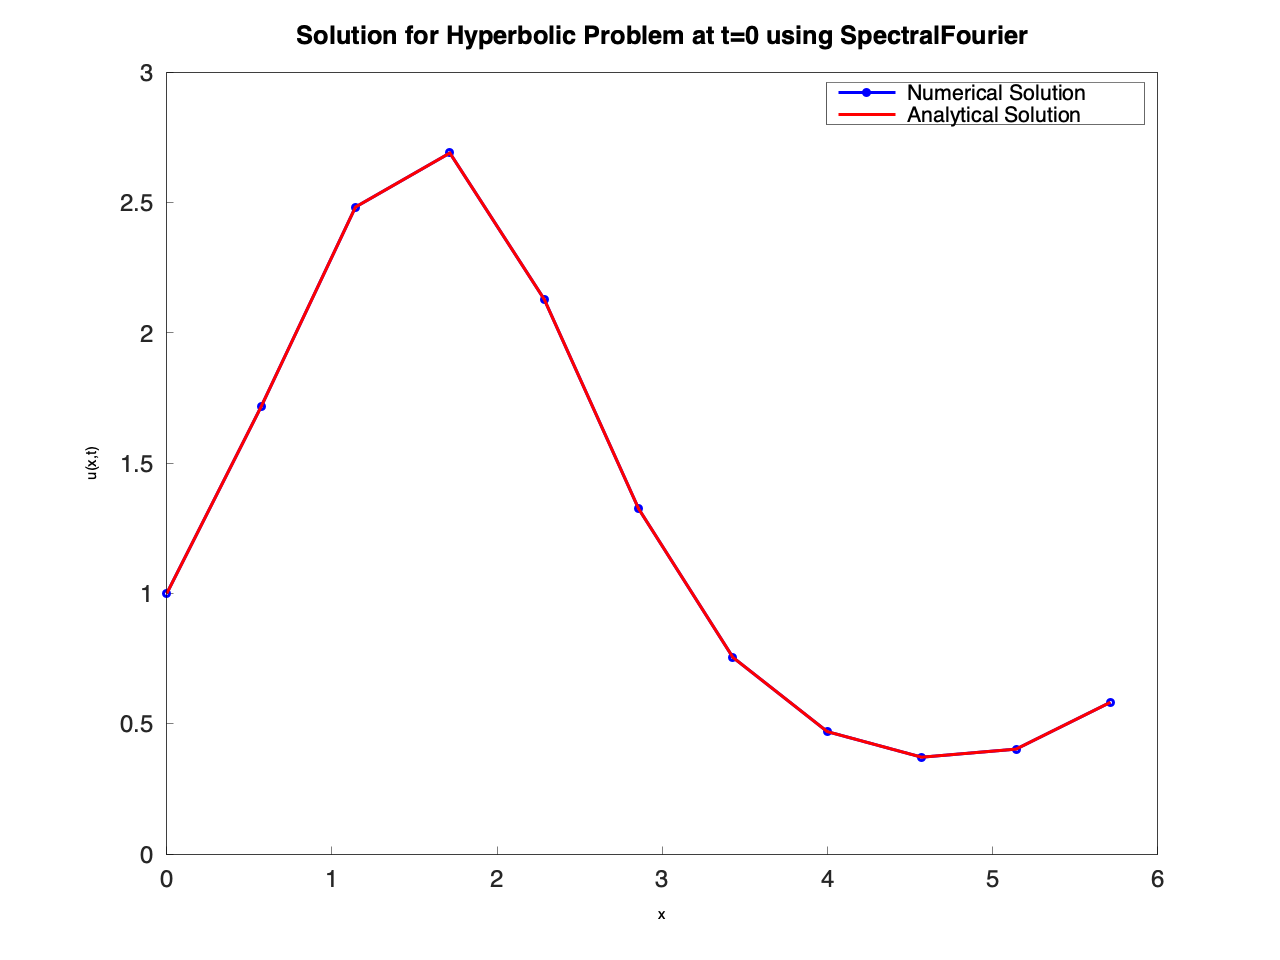
\includegraphics[width=\textwidth]{media/hyperbolic_SpectralFourier_0.png}
		\caption{Spectral Fourier at $t=0$ with $L_\infty=0.0$}
		\label{sfig:sublabel2}
	\end{subfigure}\\
	\begin{subfigure}{0.5\textwidth}
		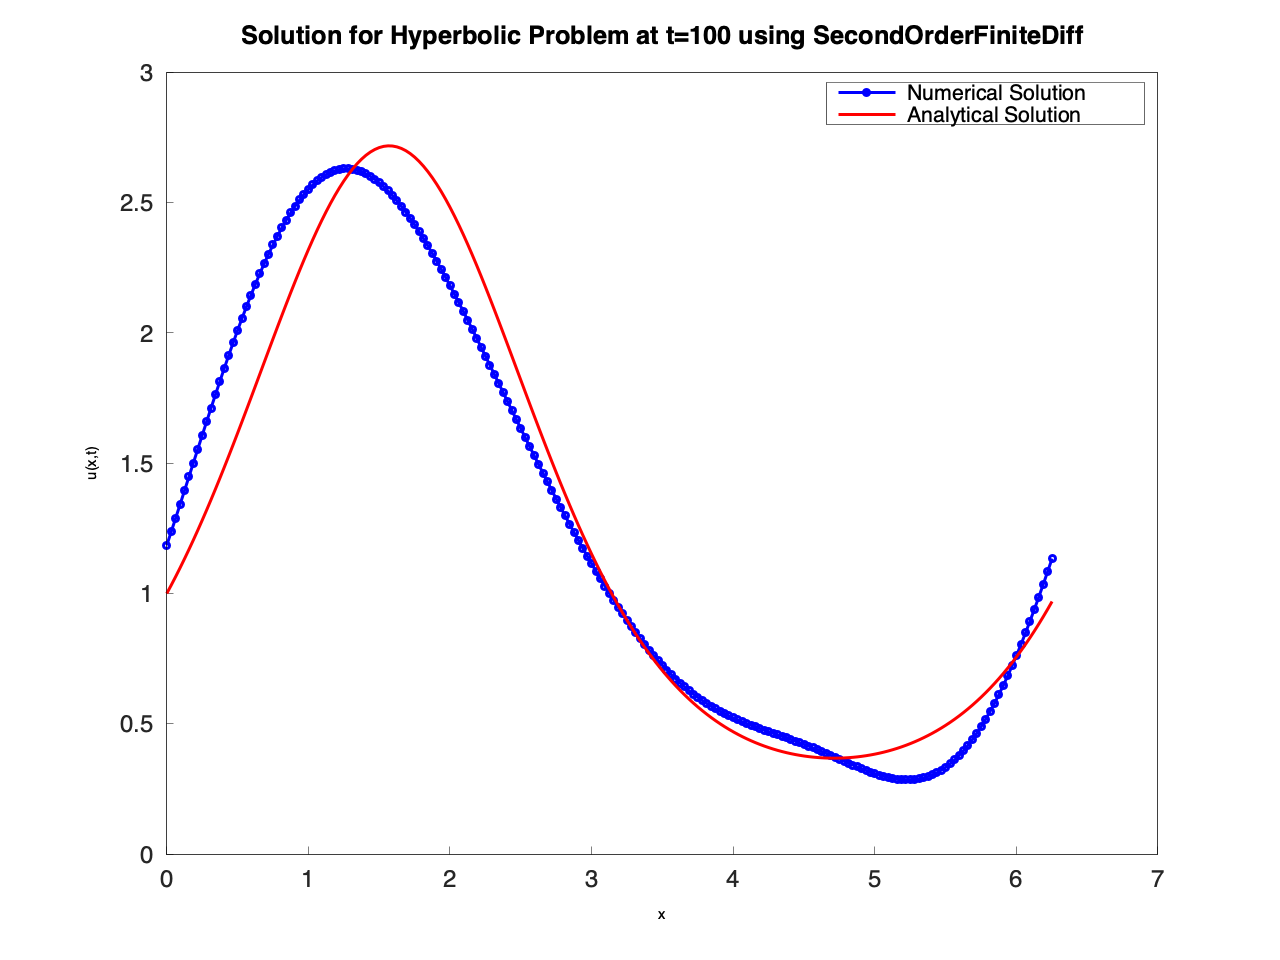
\includegraphics[width=\textwidth]{media/hyperbolic_SecondOrderFiniteDiff_100.png}
		\caption{Second Order at $t=100$ with $L_\infty = 4.0 \times 10^{-1}$}
		\label{sfig:sublabel3}
	\end{subfigure}%
	~
	\begin{subfigure}{0.5\textwidth}
		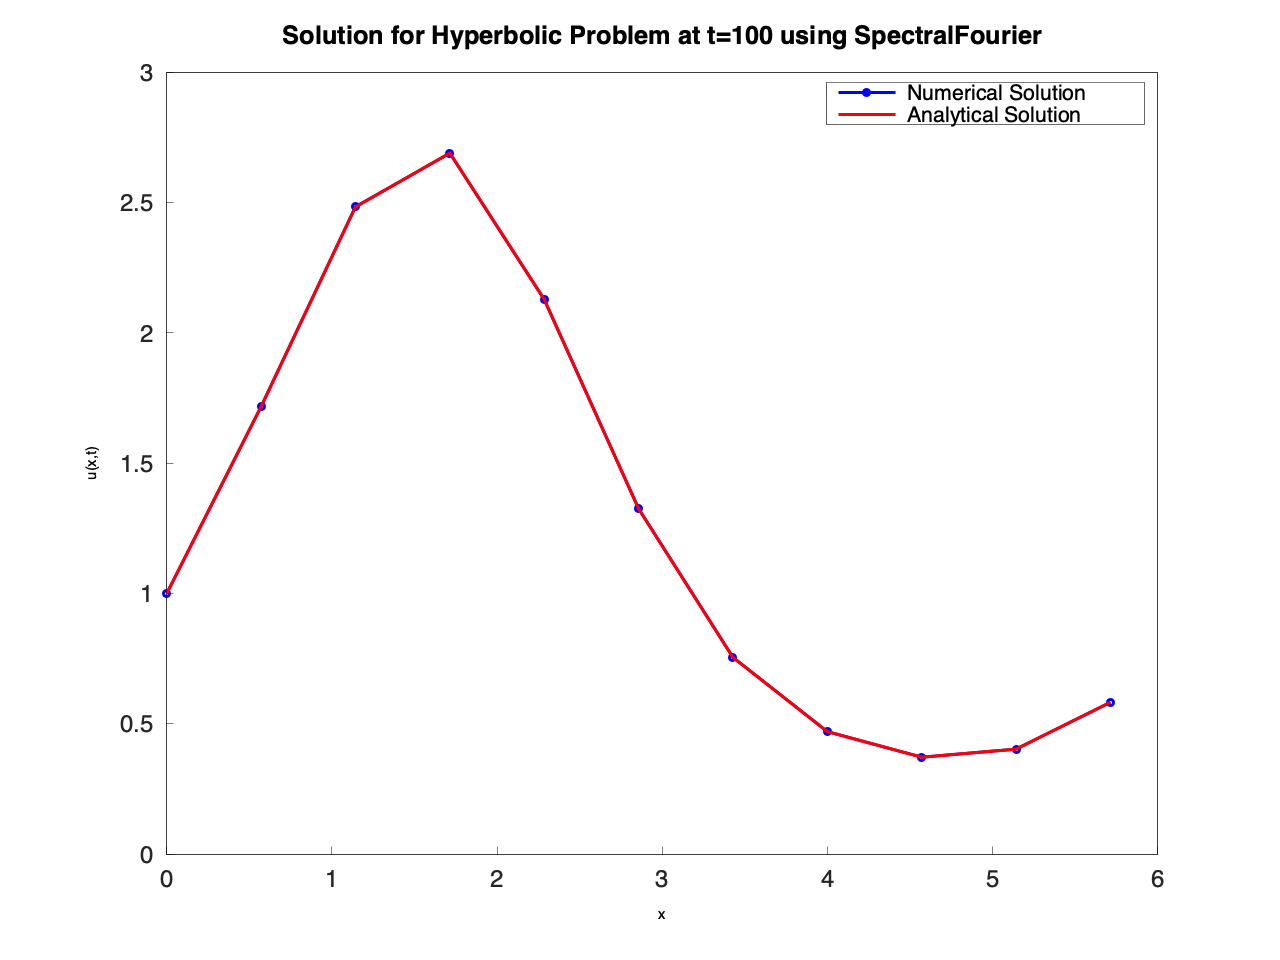
\includegraphics[width=\textwidth]{media/hyperbolic_SpectralFourier_100.png}
		\caption{Spectral Fourier at $t=100$ with $L_\infty = 1.3 \times 10^{-3}
			$}
		\label{sfig:sublabel4}
	\end{subfigure}\\
	\begin{subfigure}{0.5\textwidth}
		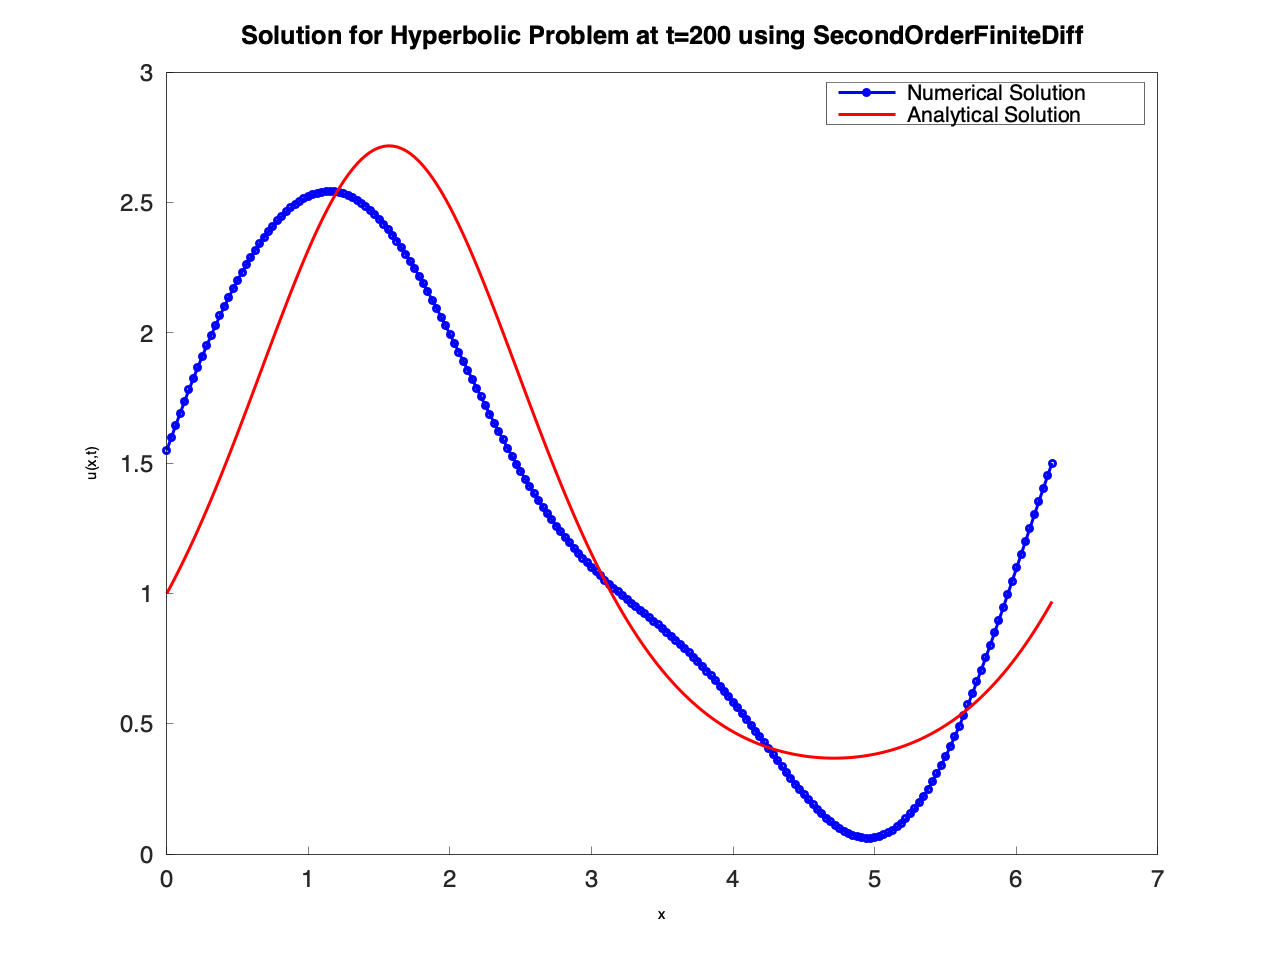
\includegraphics[width=\textwidth]{media/hyperbolic_SecondOrderFiniteDiff_200.png}
		\caption{Second Order at $t=200$ with $L_\infty = 6.3 \times 10^{-1}$}
		\label{sfig:sublabel5}
	\end{subfigure}%
	~
	\begin{subfigure}{0.5\textwidth}
		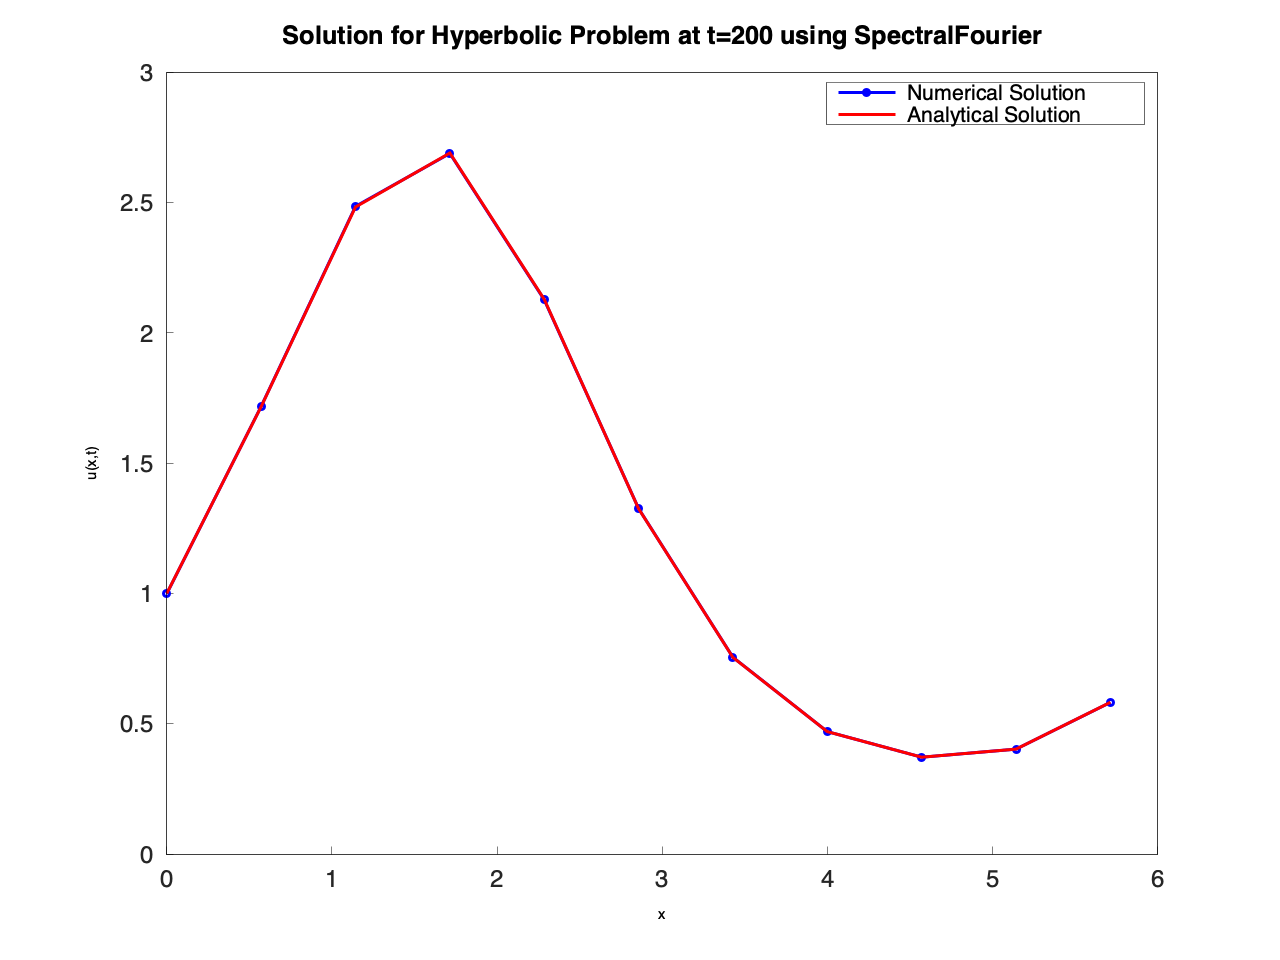
\includegraphics[width=\textwidth]{media/hyperbolic_SpectralFourier_200.png}
		\caption{Spectral Fourier at $t=200$ with $L_\infty = 2.3 \times 10^{-3}$}
		\label{sfig:sublabel6}
	\end{subfigure}

	\caption{\textbf{Comparison of Second Order Finite Difference and Spectral Fourier}
		captionText
	}
	\label{fig:figureLabel}
\end{figure}
